%--------------------
% Packages
% -------------------
\documentclass[11pt,a4paper,titlepage]{article}
\usepackage[utf8x]{inputenc}
\usepackage[T1]{fontenc}
%\usepackage{gentium}
\usepackage{mathptmx} % Use Times Font
\usepackage{amsmath}


\usepackage[pdftex]{graphicx} % Required for including pictures
\usepackage[english]{babel} % Swedish translations
\usepackage[pdftex,linkcolor=black,pdfborder={0 0 0}]{hyperref} % Format links for pdf
\usepackage{calc} % To reset the counter in the document after title page
\usepackage{enumitem} % Includes lists

\frenchspacing % No double spacing between sentences
\linespread{1.2} % Set linespace
\usepackage[a4paper, lmargin=0.1666\paperwidth, rmargin=0.1666\paperwidth, tmargin=0.1111\paperheight, bmargin=0.1111\paperheight]{geometry} %margins
%\usepackage{parskip}

\usepackage[all]{nowidow} % Tries to remove widows
\usepackage[protrusion=true,expansion=true]{microtype} % Improves typography, load after fontpackage is selected

%-----------------------
% Set pdf information and add title, fill in the fields
%-----------------------
\hypersetup{ 	
pdfsubject = {},
pdftitle = {},
pdfauthor = {}
}

%-----------------------
% Begin document
%-----------------------

\begin{document} %All text i dokumentet hamnar mellan dessa taggar, allt ovanför är formatering av dokumentet
\bibliographystyle{ieeetr}

\begin{titlepage}
  \centering
  \vspace*{2cm}
  {\Huge \textbf{\underline{CS-E4840}}}\\[0.5cm]
  {\Huge \textbf{\underline{\parbox{0.8\linewidth}{\centering Information Visualization D}}}}\\[1.0cm]
  {\Large \textbf{Assignment 3: Human Factors}} \\
  [1.0cm]
  {\Large Aleksi Kääriäinen (728971)}\\[1.0cm]
  {\Large \today}
\end{titlepage}

\section*{Introduction}
In this assignment, I have completed two visualization tasks using data relating to the SDG selected in assignment 1. Restating just for clarity, I picked SDG number 1, No poverty, for the topic of the assignments. Both tasks in this use the same dataset, that has also been used in assignments 1 and 2. The dataset includes data for the share of population living under the poverty line (daily income of US\$30) for most of the countries in the world in the time interval of years 1981-2019. The dataset is publicly available at \cite{data}.

\section{Maps and Colormaps}

In this task, I created two chorophleth maps using the poverty data. The graphs were created using \texttt{plotly}'s \texttt{choropleth} tool. Figure \ref{fig:viz1} shows the data colored with a sequential colormap, whereas figure \ref{fig:viz2} plots the normalized data using a diverging colormap. 

The data used in figure \ref{fig:viz2} was normalized with the formula:
\begin{align*}
x^{\prime} = \frac{x - \hat{x}}{\max{|x|}},
\end{align*}
where $x$ is a vecotr of real numbers, $\hat{x}$ is the mean of $x$, and $\max{|x|}$ is the maximum value of the absolute values of $x$. The normalization results in a zero-mean vector, with all values in range $[-1, 1]$. Thus figure \ref{fig:viz2} show cases the countries' relative deviation from the mean share of population living in poverty.

\begin{figure}[h]
    \centering
    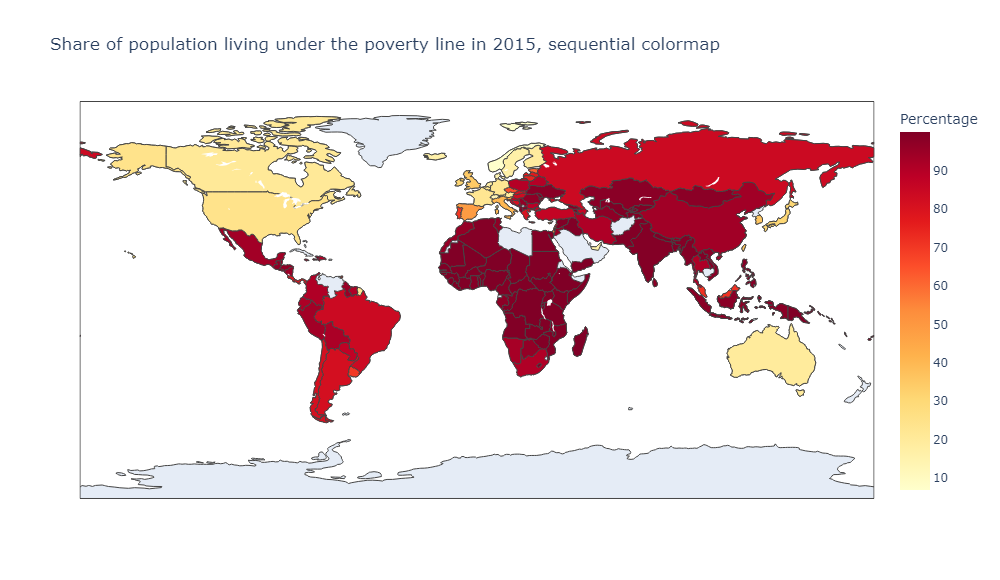
\includegraphics[width=1.0\linewidth]{reports/assignment-3/imgs/task1-1.png}
    \caption{Task 1 visualization (a)}
    \label{fig:viz1}
\end{figure}

\begin{figure}[h]
    \centering
    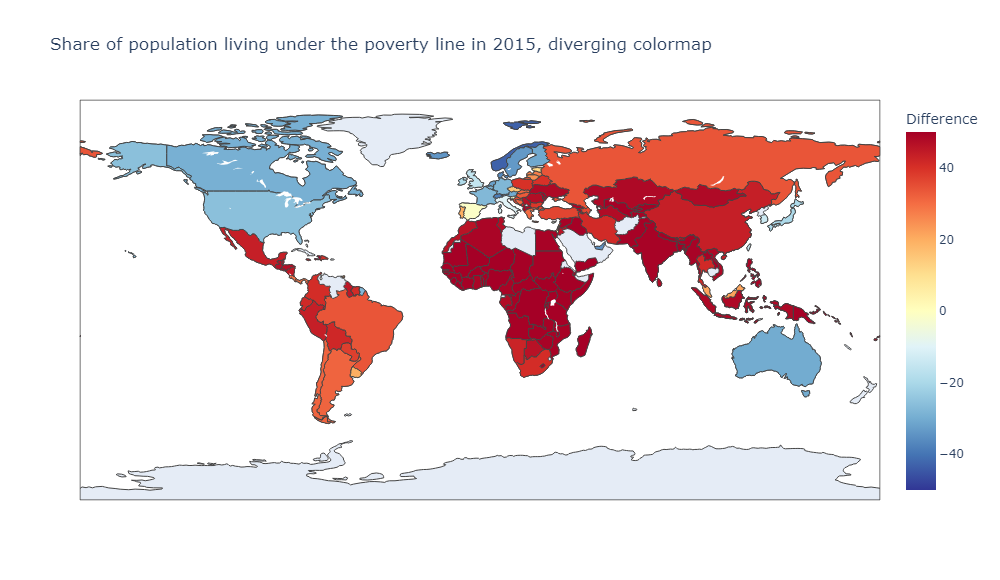
\includegraphics[width=1.0\linewidth]{reports/assignment-3/imgs/task1-2.png}
    \caption{Task 1 visualization (b)}
    \label{fig:viz2}
\end{figure}

\section{Heatmaps and Clustermaps}

\bibliography{reports/assignment-3/refs}

\end{document}